\documentclass{school-22.211-notes}
\date{February 13, 2012}

\begin{document}
\maketitle


%%%%%%%%%%%%%%%%%%%%%%%% Neutron Slowing Down and Thermalization %%%%%%%%%%%%%%%
\lecture{Slowing Down \& Thermalization in Infinite Medium} \label{slowing-down-thermalization}
The goal of this and the next section (resonant approximation) is to derive group cross sections. Thus we need to approximate the spectrum. We are going to consider: 
\begin{itemize}
\item Ignore space and angles (assuming infinite medium) and only consider the energy space. When we discuss two region heterogeneous resonant model, we are going to add some spatial dependency back in the model. 
\item Assume isotropic elastic down scattering, we get a $P(E\to E') = \frac{1}{(1-\alpha)E}$ where $E' \in [\alpha E, E]$. In lethargy space, $P(u\to u')$ is a curve pointing downwards from $0$ to $\epsilon$. 
\item Between resonances, we can assume the cross section is flat, thus we get the 1/E spectrum again. 
\item In handling the resonances, we introduce NR (resonance is so narrow that a scattering can take us out of the resonance and we can ignore resonances in a sense) and WR (resonance is so large that we are stuck inside for a while, thus the reaction rate is constant). 
\item Then we add back in spatial dependency, and discuss the simpliest two region approximation.
\end{itemize}


\topic{Summary: Reuss Ch 7 Neutron Slowing Down}
\begin{enumerate}
\item Decouple absorption and scattering is possible because absorption is complicated at lower energies, whereas scattering is the opposite (b/c inelastic and anisotropic aspects). 

\item Elastic vs. inelastic: elastic scattering has no threshold, making it the most important one in neutron slowing down. Inelastic scattering has a threshold of a few MeV for light nuclei, and a few tens of keV for heavy nuclei, making it mainly observed in the fuel materials particularly \ce{^{238} U}. 

\item In Lab system, laws of elastic collision: 
  \begin{align}
    \frac{E_{nf}}{E_{ni}} &= \frac{A^2 + 1 + 2A \cos \theta}{(A+1)^2} = \frac{1}{2} \left[ 1 + \alpha + (1-\alpha) \cos \theta \right] \\
    \cos \psi &= \frac{1 + A \cos \theta}{\sqrt{A^2 + 1 + 2A \cos \theta}} \\
    \alpha &= \frac{(A-1)^2}{(A+1)^2} = \mbox{min ratio between final n energy and initial} 
  \end{align}

\item In CMCS, scattering is isotropic in solid angle $\Omega$(except very high energy), which implies that $\cos \theta$ is uniform, and $E_{nf}$ is uniform:

  \begin{align}
    P(\theta) \dtheta &= \frac{1}{2} \sin \theta \dtheta = \frac{1}{2} \derivative |\cos \theta| \\
    P(E) \dE &= \frac{\dE}{(1-\alpha) E_i} 
  \end{align} 

\item In Lab system, scattering towards the front it favored. The mean of $\cos \psi$ is $\mu = \expect{ \cos \psi} = \frac{2}{3A}$. 

\item Lethargy, a unitless measurement of energy (the idea comes from laws of elastic collision governs an energy ratio):
  \eqn{ u = \ln \frac{E_{\mathrm{ref}}}{E} }
Notice as time goes, neutrons slow down, $u$ increases, making it like a measure of the age of the neutrons. Then we know that the uniform distribution of energy becomes a decreasing exponential distribution for lethargy gain: 
\begin{align}
w &= u_f - u_i = -\ln \left[ \frac{1}{2} ( 1 + \alpha + (1-\alpha) \cos \theta ) \right] \\
w_{min} &= 0 \\
w_{max} &= \epsilon = -\ln \alpha \\
P(w) \dw &= \frac{e^{-w}}{1 - \alpha} \dw \\
\expect{w} &= \xi = 1 - \frac{\alpha \epsilon}{1 - \alpha} 
\end{align}
$\xi$ is like the efficiency of slowing down by a nucleus. That is, neutrons advance by $\xi$ lethargy units on average at each collision. Then to overcome the total lethargy interval $U = \ln \frac{E_0}{E_1}$, the number of collisions needed is:
\eqn{ n = \frac{U}{\xi} }
\begin{table}
  \centering
  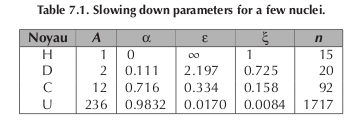
\includegraphics[width=3in]{images/sl-d/slowing-down-parameter.png}
  \caption{Slowing Down parameters}\label{slowing-down-parameter}
\end{table}

\item Moderating power is the best measure of a material's ability to slow down neutrons. It has two forms:
\eqn{\mbox{per atom basis} = \xi \sigma_s \fsp \fsp \fsp \mbox{per volume basis} = \xi \Sigma_s   }
A good moderating material should have: high slowing down (hence light nuclei), low capture (D, Be, C), moderating power (take into account both high slowing down and high scattering xs). Water has the highest moderating power, but it requires an enriched fuel (around 1\%). 
\begin{table}
  \centering
  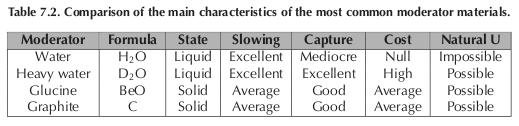
\includegraphics[width=4in]{images/sl-d/moderator-comparison.png}
  \caption{Comparison of Characteristics of Moderators}\label{moderator-comparison}
\end{table}

\item Laws of inelastic collision. Elastic scattering is important for moderators because they are light; inelastic scattering is important for heavy materials like the fuel because they have almost no elastic collision. Minimum energy of the neutron for an inelastic collision is:
\eqn{ E_{\mathrm{threshold}} = \frac{A+1}{A} Q } 

\item Slowing down equations: a simplified Boltzmann equation performing neutron counts that depends on one variable, either velocity or energy or lethargy. We pick lethargy. Then we assume an infinite, homogeneous medium with a source uniform in space and time. 

\item First form of the slowing down equation (7.1.9):
  \begin{align}
    \rho(u) \du 
    &= \mbox{arrival density} = \begin{array}{l}
      \mbox{\# neutrons arriving per time and per volume} \\
      \mbox{in d$u$ between $u$ and $u + \du$ following a scattering to $u'$} 
      \end{array} \\
    &= \overbrace{\int_{-\infty}^u \Sigma_s (u') \Phi(u') \du'}^{\textcircled{1}} \overbrace{ P(u'\to u) \du }^{\textcircled{2}} \\
    \textcircled{1} &= \mbox{\# neutrons travelling in du' and scattered per time and per volume} \\
    \textcircled{2} &= \mbox{probability a neutron scattered at u' will be transferred in du} \\
    \rho(u) &= \int_{-\infty}^u \Sigma_s (u'\to u) \Phi(u') \du' \\
    S(u) + \rho(u) &= \boxed{S(u) + \int_{-\infty}^u \Sigma_s (u'\to u) \Phi(u') \du  = \Sigma(u) \Phi(u) }
  \end{align}
  In the specific case of COM isotropic, monatomic elastic slowing down, the transfer probability is:
  \eqn{P(u'\to u) = P(u\to u') = \frac{e^{-(u-u')}}{1-\alpha} }
\item Decay of neutron spectrum by successive scattering events (7.2.2): producing spectrum by adding up successive scattering events;
\item Slowing down without absorption (7.2.3). Asymptotic value of flux: 
  \eqn{ \Phi_{as} (u) = \frac{S}{\xi \Sigma_s(u)} }
  If we plot flux vs. lethargy, all isotopes would fluctuate (Placzek transient) before reaching the asymptotic flux value, except H which immediately reaches $\Phi_{as}$. 
\item Slowing down in hydrogen (7.2.4): uses Green's function; the Dirac distribution compensates for the source in the equation; the Heaviside step function makes sure the neutrons scattered at least once scattered beyond, not below, the original lethargy. 
\item Slowing down with resonance absorptions (which is low energy) (7.2.5): we can approximate resonance absorption of the following types
  \begin{enumerate}
    \item Black resonance trap: 
      \eqn{ 1 - p = \int_0^{\gamma} \int_{u-\epsilon}^0 \du' \frac{1}{\xi} \frac{e^{-(u-u')}}{1 - \alpha} = \frac{1 - e^{-\gamma} - \alpha \gamma}{\xi (1-\alpha)}  }
      when $\gamma$ is small, we can simplify the above to be $1 - p = \frac{\gamma}{\xi}$. 
    \item Narrow grey resonance trap:
      \eqn{ 1 - p  = \int_{\mathrm{trap}} \frac{\Sigma_a(u)}{\Sigma_t(u)} \frac{\du}{\xi} }
    \item A set of narrow grey resonance traps: we express each resonance in exponential form, and find the product of them:
      \begin{align}
        p_i &= 1 - \int_i \frac{\Sigma_a(u)}{\xi \Sigma_t (u)} \du = \exp \left[ -\int_i \frac{\Sigma_a(u)}{\xi \Sigma_t(u)} \du \right] \\
        p &= \prod_i p_i = \exp \left[ - \Sum_i \int_i \frac{\Sigma_a(u)}{\xi \Sigma_t(u)} \du \right]
      \end{align}
    \item General expression:
      Because the integrated function is zero outside of the resonance traps, we can simply write,
      \eqn{p =  \exp \left[ - \int \frac{\Sigma_a(u)}{\xi \Sigma_t(u)} \du \right] }
      This is the general expression for resonance escape probability. 
  \end{enumerate}
\item Slowing down with low, slowly varying absorption (which is high energy) (7.2.6). 

  \begin{enumerate}
  \item Greuling-Goertzel approximations for slow and gradually varying absorption: 
  \item Wigner approximation for resonance absorption: 
  \end{enumerate}
\end{enumerate}

%%%%%%%%%%%%%%%%%%%%%%%%%%%% Ch 9 %%%%%%%%%%%%%%%%%%%%%%%%%%%%%%%%
\topic{Summary: Reuss Ch 9 Thermalisation of Neutrons}
\begin{enumerate}
\item For monatomic gas, there is thermal agitation and no chemical bonds, we can approximaet with Maxwell distribution. 
\item For any thermaliser, the neutron spectrum at equilibrium and in the absence of absorption (or with low capture) would be a Maxwell spectrum. A Maxwell spectrum depends on $E, kT$. 
\item Microreversibility principle/detailed balance: at equilibrium and with no absorption, the number of transfers by diffusion from $\dE$ to $\dE'$ as transfers in the other direction from $\dE'$ to $\dE$. 
\item Scattering equation (9.1.4): 
\eqn{ \Sigma_s(E', E, \mu) = \Sigma_s (E') P(E' \to E) P(\mu) = C^{te} \sqrt{\frac{E}{E'}} \exp \left[\frac{E'-E}{2kT} \right] S(\alpha, \beta)  }
\item Thermalisation equation (9.1.5): 
  \eqn{ \int_0^{E_{\mathrm{cutoff}}} \Sigma_s (E') \Phi(E') \dE' P(E' \to E) + \overbrace{\int_{E_{\mathrm{cutoff}}}^{\infty} \Sigma_s(E') \Phi(E') \dE' P(E'\to E)}^{S_{\mbox{slow-down}}(E)} = \Sigma_t(E) \Phi(E) }
  and the slow-down equation, 
  \eqn{ \int_{-\infty}^{u} \Sigma_s (u') \overbrace{P(u' \to u)}^{\frac{\exp(-(u-u'))}{1 - \alpha}} \Phi(u') \du' + S(u) = \Sigma_t(u) \Phi(u) }
  The two are similar, except:
  \begin{enumerate}
  \item The slowing down equation only down scatters, whereas thermalisation equation can transfer energies in both directions. The upper boundary $E_{\mathrm{cutoff}}$ is the energy separating the thermalization domain from the slowing down domain. 
  \item The `source' in the thermalisation equation $S_{\mbox{slow-down}}(E)$ is not a true source; it is a density of arrival at energies below the cutoff energy due to scattering events occurring in the last part of the slowing down domain and transferring the neutron beyond the cutoff energy in the thermalisation domain. 
  \end{enumerate}
\item Thermal Spectrum(9.2): it is approximately reasonable well by Maxwell distribution, except,
  \begin{itemize}
    \item $0\sim 2kT$: real thermal spectrum is smaller due to absorption of neutrons;
    \item $2kT$ and above: Maxwell spectrum approaches zero quickly, whilst the real density falls slightly but remains significant, due to the `slowing down queue:' neutrons coming from high energies slow down and enter the thermal domain, compensating for the disappearances by absorption. 
  \end{itemize}
\item Comparing MOX and UOX spectrum: the two are close for the fast and epithermal domains, because they essentially have the same quantity of moderator, U238, and cladding. Whereas in the thermal domain, the number of neutrons in MOX is lower by a factor of 4 because of the high absorption by MOX fuel of thermal neutrons. 
\item Average cross section (9.2.3): 
  \eqn{ \bar{\sigma} = \frac{\int \sigma(E) \Phi(E) \dE}{\int \phi(E) \dE} }
  \uline{Example: calculate the average xs for a Maxwell spectrum and a 1/v xs.} 
  \eqn{ \bar{\sigma} = \frac{\sqrt{\pi}}{2} \sigma(v_0) = \frac{\sqrt{\pi}}{2} \sqrt{\frac{293}{T}} \sigma_{2200} }
  where $\frac{\sqrt{\pi}}{2}$ is the average of $x = v/v_0$ on a Maxwell spectrum, and also the average of $1/x$. 
\item Heterogeneous Configurations (9.2.4):
  \begin{align}
    V_f R_f \Phi_f P_{ff} + V_m (R_m \Phi_m + S_{\mathrm{sl-d}} ) P_{mf} &= V_f \Sigma_f \Phi_f \\
    V_fR_f \Phi_f P_{fm} + V_m(R_m \Phi_m + S_{\mathrm{sl-d}}) P_{mm} &= V_m \Sigma_m \Phi_m 
  \end{align}
\item Approximate thermal neutron speeds(9.3.1): assume absorption xs are 1/v and scattering xs are constant, we can approximate
  \eqn{ v = 2200 \m/\s \sqrt{\frac{T}{293.15}} } 
\item Thermal utilisation factor (9.3.2): the fraction of thermal neutrons absorbed in the fuel,
  \eqn{ f &= \frac{V_f \Sigma_{a,f} \Phi_f}{V_f \Sigma_{a,f} \Phi_f + V_m \Sigma_{a,m} \Phi_m + \cdots}, & \frac{1}{f} - 1 &= \underbrace{\frac{V_m}{V_f}}_{\mbox{moderation ratio}}
    \overbrace{\frac{\Phi_m}{\Phi_f}}^{\mbox{disadvantage factor}} \frac{\Sigma_{a,m}}{\Sigma_{a,f}}   } 
\item Reproduction factor $\eta$ (9.3.3):
  \eqn{ \eta = \frac{\nu \Sigma_{f,f}}{\Sigma_{a,f}} }
\end{enumerate}
%%%%%%%%%%%%%%%%%%%%%% end of Ch 9 %%%%%%%%%%%%%%%%%%%%%%%%%%%%%



\clearpage
%%%%%%%%%%%%%%%%%%%%%% start of MC %%%%%%%%%%%%%%%%%%%%%%%%%%%%%
\topic{A MC Infinite Medium Model}
This Monte Carlo Model we develope for this chapter and next chapter is for infinite medium. 
\subtopic{Calculating Isotopic Importance}
Given an infintie medium LWR with volume fraction listed in Table.~\ref{volume-fraction}, we can calculate isotopes' number densities: 

\begin{table}[ht]
  \centering
  \begin{tabular}{|c|c|c|c|} \hline
    Reactor & Fuel & Coolant \& Moderator & Structural  \\ \hline \hline
    PWR & 35\% & 55\% & 10\% \\ \hline
    CANDU6 & 5\% & 85\% & 10\%  \\ \hline
    HTGR & 5\% & 90\% & 2\% \\ \hline
    SFR & 60\% & 30\% & 10\% \\ \hline
  \end{tabular}
  \caption{Volume Fraction/Isotopic Importance of Reactor Materials for Typical LWRs} \label{volume-fraction}
\end{table}

\begin{align}
N^H_c &= 0.55 \times 1 \g/\cm^3 \frac{N_{AV} \mathrm{molecule}/\mol}{18 \g/\mol} 2/\mathrm{molecule}  = 3.68 \times 10^{22} \\
N^O_c &= 0.55 \times 1 \g/\cm^3 \frac{N_{AV} \mathrm{molecule}/\mol}{18 \g/\mol} 1/\mathrm{molecule}  = 1.84 \times 10^{22} \\
N^O_f &= 0.35 \times 10 \g/\cm^3 \frac{N_{AV} \mathrm{molecule}/\mol}{270 \g/\mol} 2/\mathrm{molecule}  = 1.56 \times 10^{22} \\
N^{238}_f &= 0.95 \times 0.35 \times 10 \g/\cm^3 \frac{N_{AV} \mathrm{molecule}/\mol}{270 \g/\mol} 1/\mathrm{molecule}  = 1.48 \times 10^{22} \\
N^{235}_f &= 0.05 \times 0.35 \times 10 \g/\cm^3 \frac{N_{AV} \mathrm{molecule}/\mol}{267 \g/\mol} 1/\mathrm{molecule}  = 0.079 \times 10^{22} \\
N^{Zr} &= 0.10 \times 6.6 \g/\cm^3 \frac{N_{AV} \mathrm{molecule}/\mol}{90 \g/\mol} 1/\mathrm{molecule}  = 0.56 \times 10^{22} 
\end{align}
That is, in a typical LWR the relative number densities come out to be around: 
\eqn{\boxed{H = 1, O = 1, U238 = 0.4, U235 = 0.02, Zr = 0.15   }}
Notice \hi{hydrogen's and oxygen's number densities are about the same.} 


\subtopic{Abtracting Cross Sections}
See Figure~\ref{scatter-xs}, Figure~\ref{capture-xs} for common cross sections. Notice resonance absorption and scattering tend to line up in terms of energy. 

\uline{Practice: Why can we use sodium as coolant if its capture cross section is so high?}  

\textbf{Answer:} Sodium has a high capture xs in thermal range, and a small capture xs in fast range. But we can still build a thermal reactor with water as moderator and sodium as coolant, as long as sodium's volume is lower than that of the H. 


\clearpage
%%%%%%%%%%%% Elastic Scattering %%%%%%%%%%%%%%%%%%%%%%
\subtopic{High Energy: Elastic Scattering}
For high energy, we assume no absorption and scattering is isotropic in COM (target at rest in Lab system). Then we arrive at some important parameters/properties: 
\begin{enumerate}
\item After each collision, the minimum final energy is,
\eqn{ \boxed{ \alpha = \frac{E_{\mathrm{min}}}{E_0}  = \left( \frac{A-1}{A+1} \right)^2 } }

\item Mean log energy decrement:
\eqn{ \boxed{ \zeta = 1 + \frac{\alpha \ln(\alpha)}{1 - \alpha}  }  }
Examples: $\zeta_{H} = 1, \zeta_D = 0.725, \zeta_C = 0.158, \zeta_U = 0.0084$. \hi{$A \up, \zeta \down$.} 

\item The number of collisions required to slow a particle from $E_2$ to $E_1$ is: 
\eqn{ \boxed{ n = \frac{\ln(E_2 / E_1)}{\zeta} }  }
Examples: for $E_2 = 2\times 10^6 \eV, E_1 = 0.1 \eV$, the number of collisions is: $n_H = 17, n_D = 23, n_C = 106, n_U = 2000$. 

\item Flux vs. energy:
\begin{figure}[ht]
  \centering
  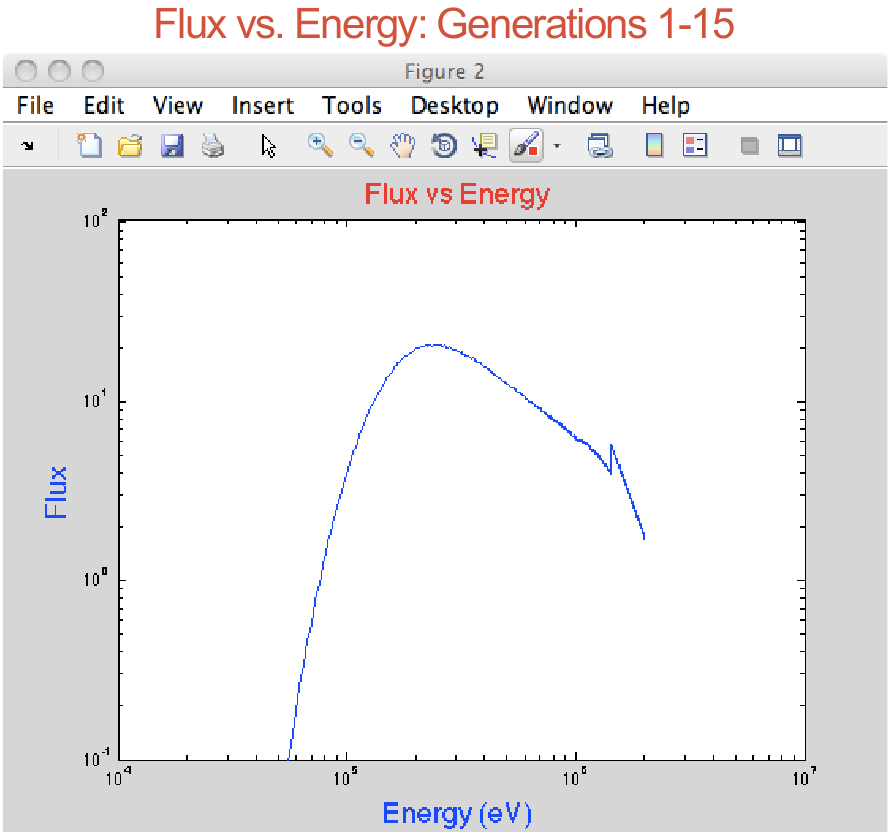
\includegraphics[width=3in]{images/sl-d/flux-vs-energy-1.png}
  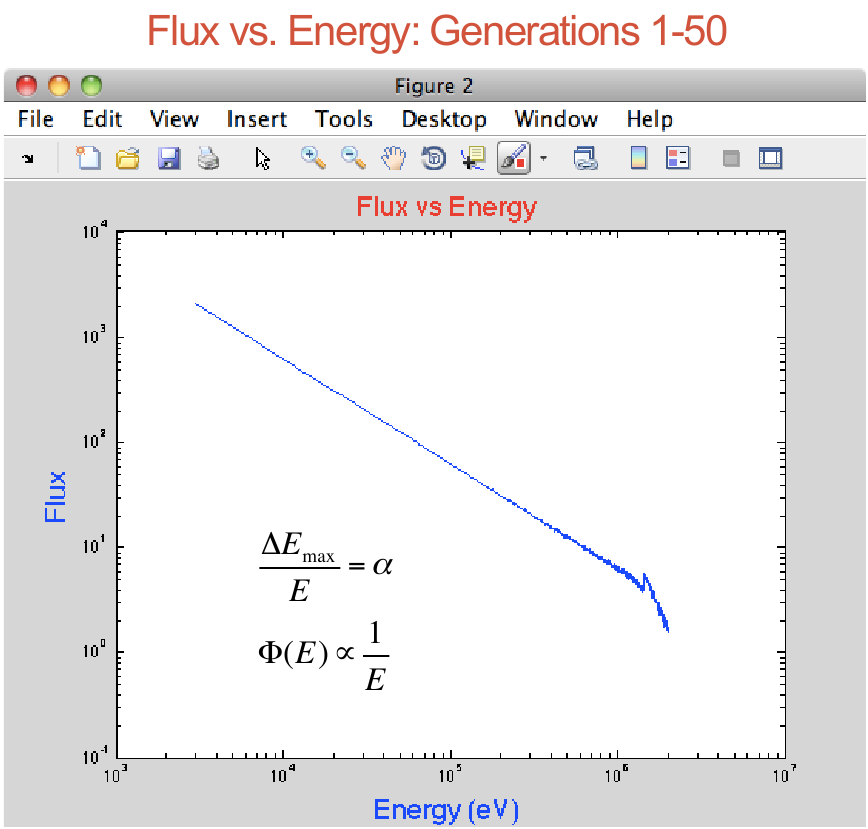
\includegraphics[width=3in]{images/sl-d/flux-vs-energy-2.png}
  \caption{Flux vs. Energy} \label{fve}
\end{figure}

There are two ways to understand flux here. 
\begin{itemize}
\item Particle based: we let all the neutrons to scatter till death; then for each energy interval, if we add up the number of neutrons with energies in that interval; we get the flux corresponding to each interval.  
\item Generation based (as in Fig.~\ref{fve}): we let each neutron scatter once in each generation, save all the number of neutrons vs. energy data, and add up all the generations, this would effectively give us flux vs. energy as well. Notice with insufficient number of generations (left plot), the flux tails down at lower energies, meaning that some neutrons are not slowed down entirely yet. With sufficient number of generations (right plot), we get a \hi{1/E spectrum} for COM elastic scattering only. 
\end{itemize}

\item Flux vs. lethargy: as in Fig.~\ref{fvl}, flux is a constant in lethargy space. 
\begin{figure}[ht]
  \centering
  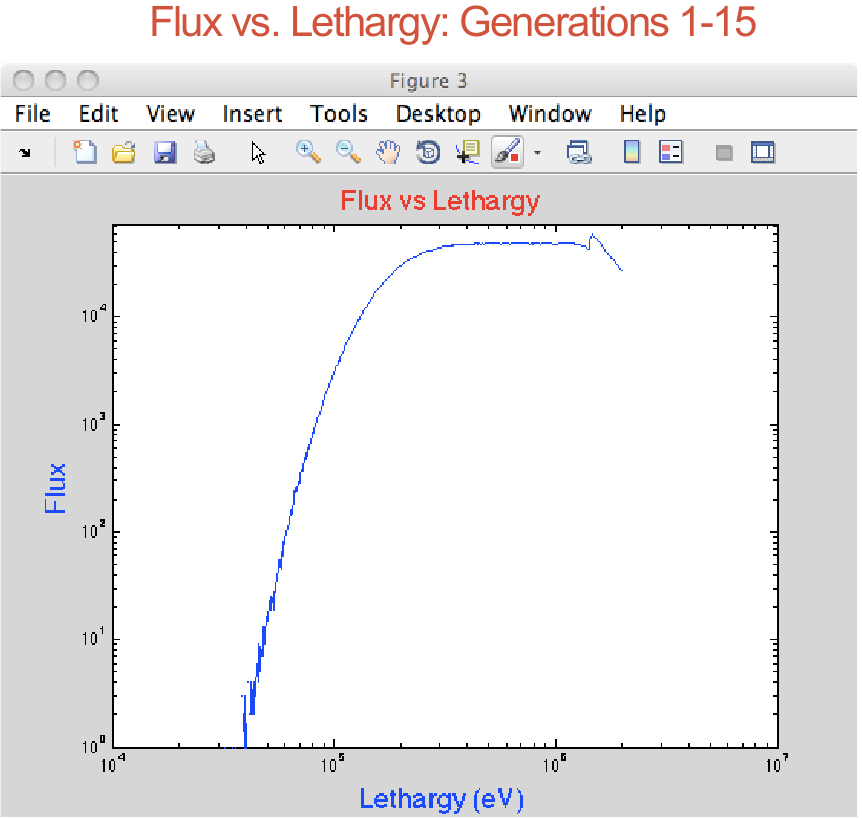
\includegraphics[width=3in]{images/sl-d/flux-vs-lethargy-1.png}
  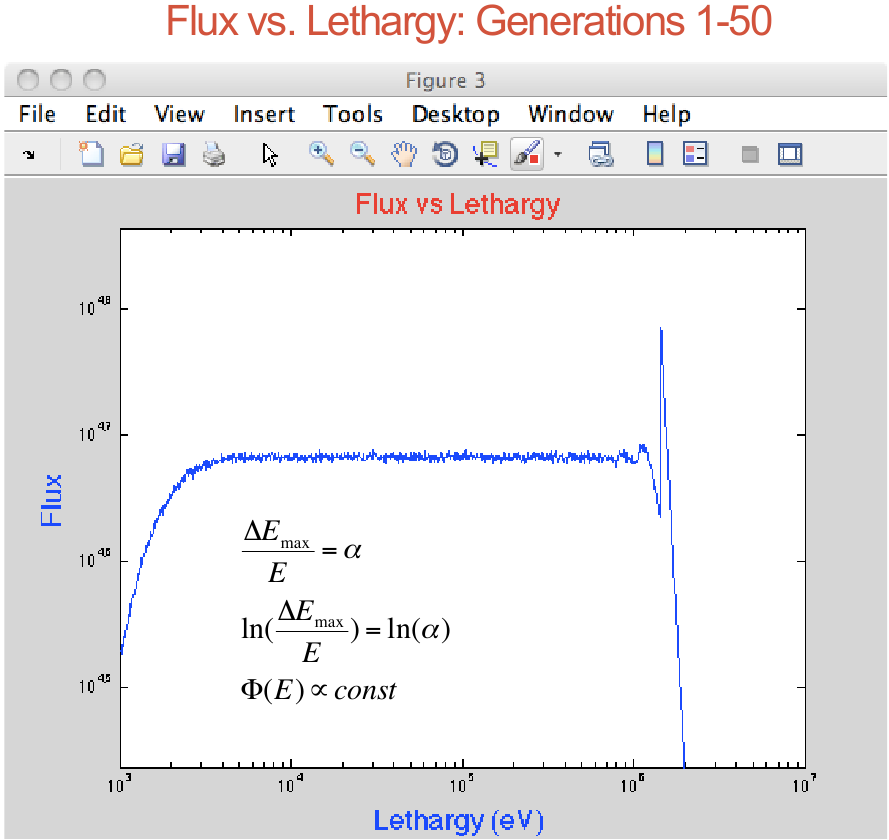
\includegraphics[width=3in]{images/sl-d/flux-vs-lethargy-2.png}
  \caption{Flux vs. Lethargy} \label{fvl}
\end{figure}

Caution about number of bins: When we are plotting, we are really plotting the expectation value of the numbers of neutrons. 

\uline{Practise: how many neutrons would there be at x energy level?}  

\textbf{Answer:} zero. So the bins have to be fine enough to see the details, but not too fine that the bins got no more neutrons. 
\end{enumerate}


\clearpage
\subtopic{High Energy: Add Fission Emission Spectrum $\chi$}
We model the fission emission spectrum $\chi(E)$ as a Maxwell spectrum:
\eqn{ \chi(E) \dE = \frac{2\pi}{(\pi T)^{3/2}} \sqrt{E} \exp\left( - \frac{E}{T} \right) \dE }
Simulation: constructing a cdf for Maxwell distribution (when constructing any cdf, it is a good practice to sample immediately and double check with the pdf); for each neutron, generate a random number $\xi \in [0,1]$, and use $\xi = cdf(E)$ to reverse-lookup for $E$, and this is the fission emission energy of that neutron. 

Characteristics of spectra after adding in $\chi(E)$ (caution: Fig.~\ref{spe1} is plotted with $x$-axis being energy, but it is still in lethargy space): 
\begin{enumerate}
\item The spectrum is independent on the number of incoming neutrons; 

\item For one specie, the spectrum is independent of its cross section; for two species, only the relative cross section matters. 

\item The effect of $\chi(E)$: smooth out the shart edge at the highest energy cutoff (Fig.~\ref{spe1} middle plot).

\item Fission source peak: so far we reach a constant spectrum in lethargy. To obtain the fission source peak around 2 MeV, we have to divide the flux count by the hydrogen cross section:
  \eqn{\phi(E) \propto \Sum_N \Sum_g N_g^n \tau_g^n = \Sum_n \Sum_g N_g^n \frac{1}{\Sigma(E_g^n)}   }
  Recall the hydrogen scattering cross section decreases from 0 to 1 eV, stays constant between 1 eV to 10 keV, and decreases again afterwards. In the fast energies, the decreased hydrogen absorption cross section increases the flux, causing the 1.7 MeV peak. 
\end{enumerate}

\begin{figure}[ht]
  \centering
  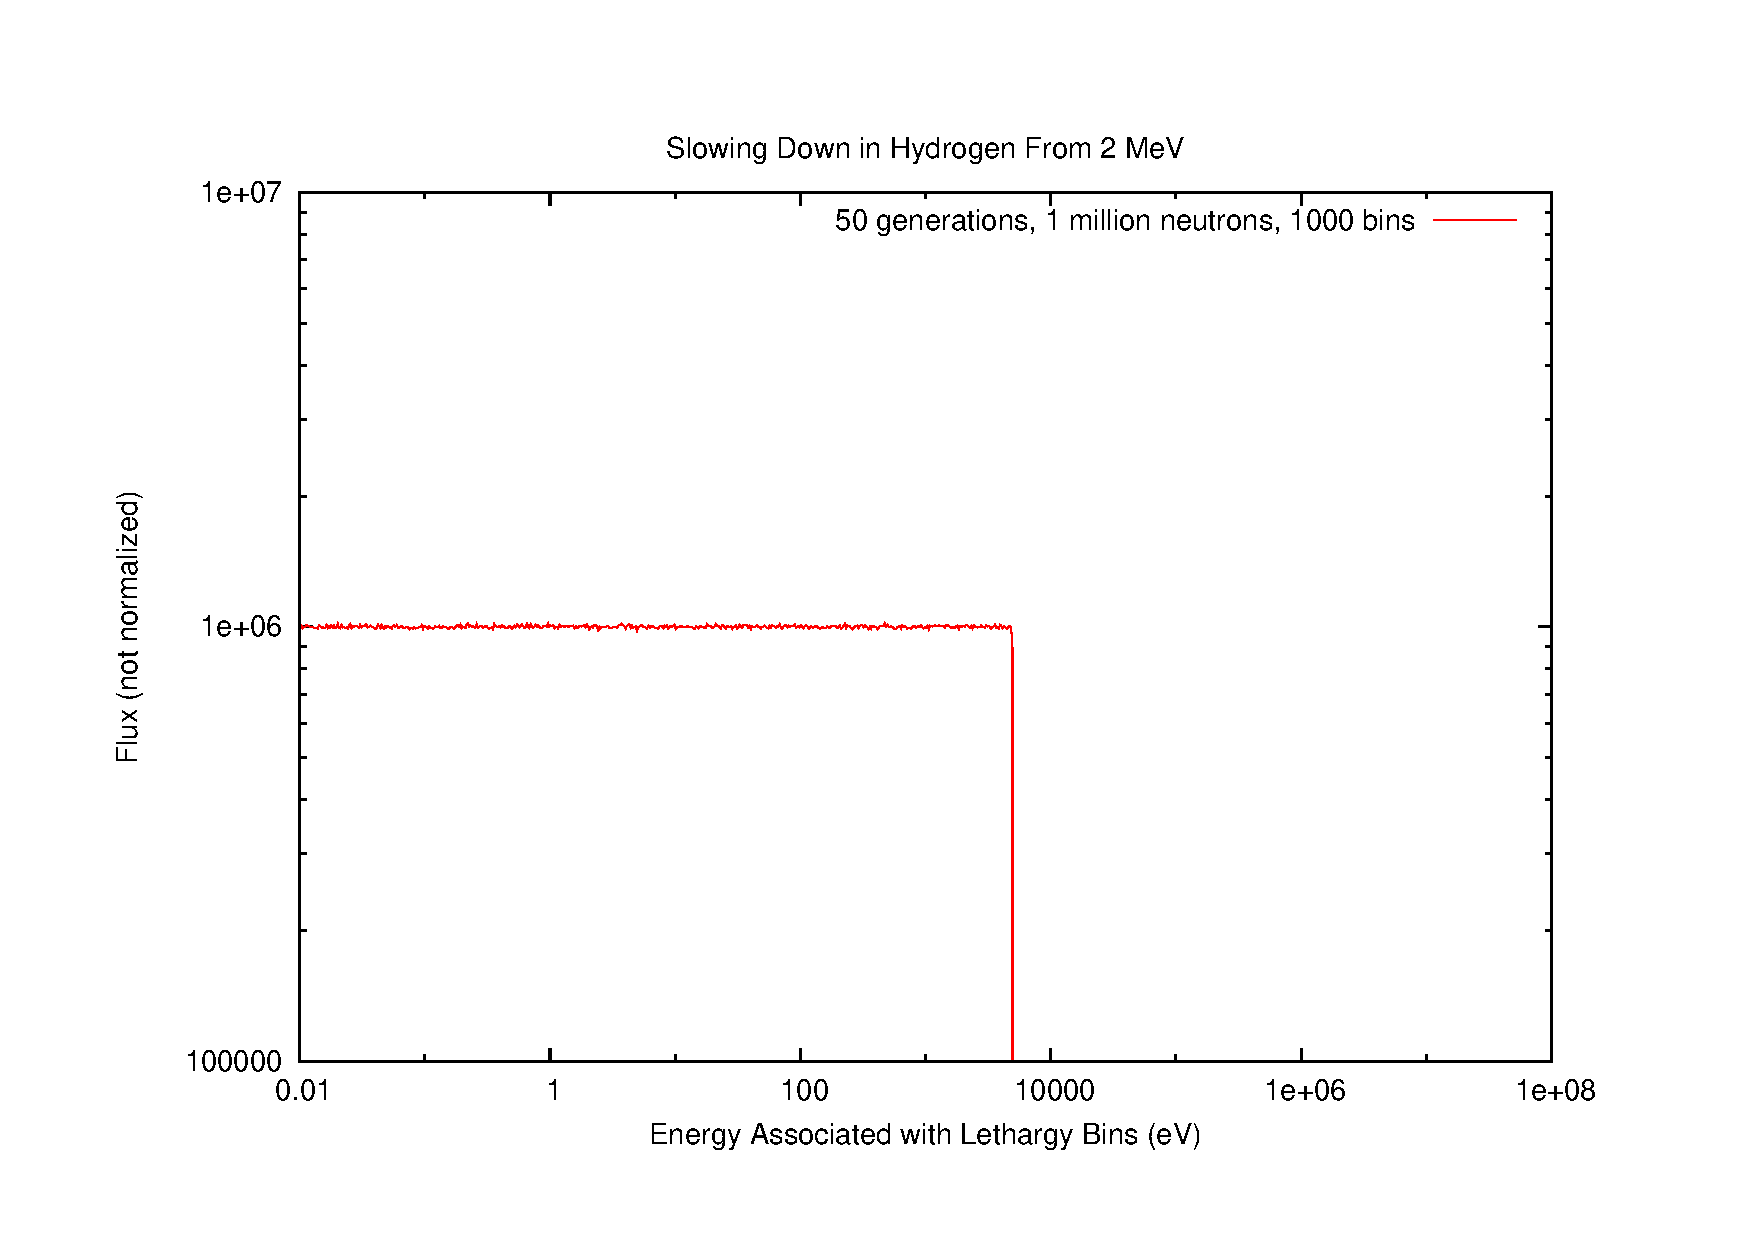
\includegraphics[width=4in]{images/sl-d/spec-1.uncrop.pdf}
  \\
  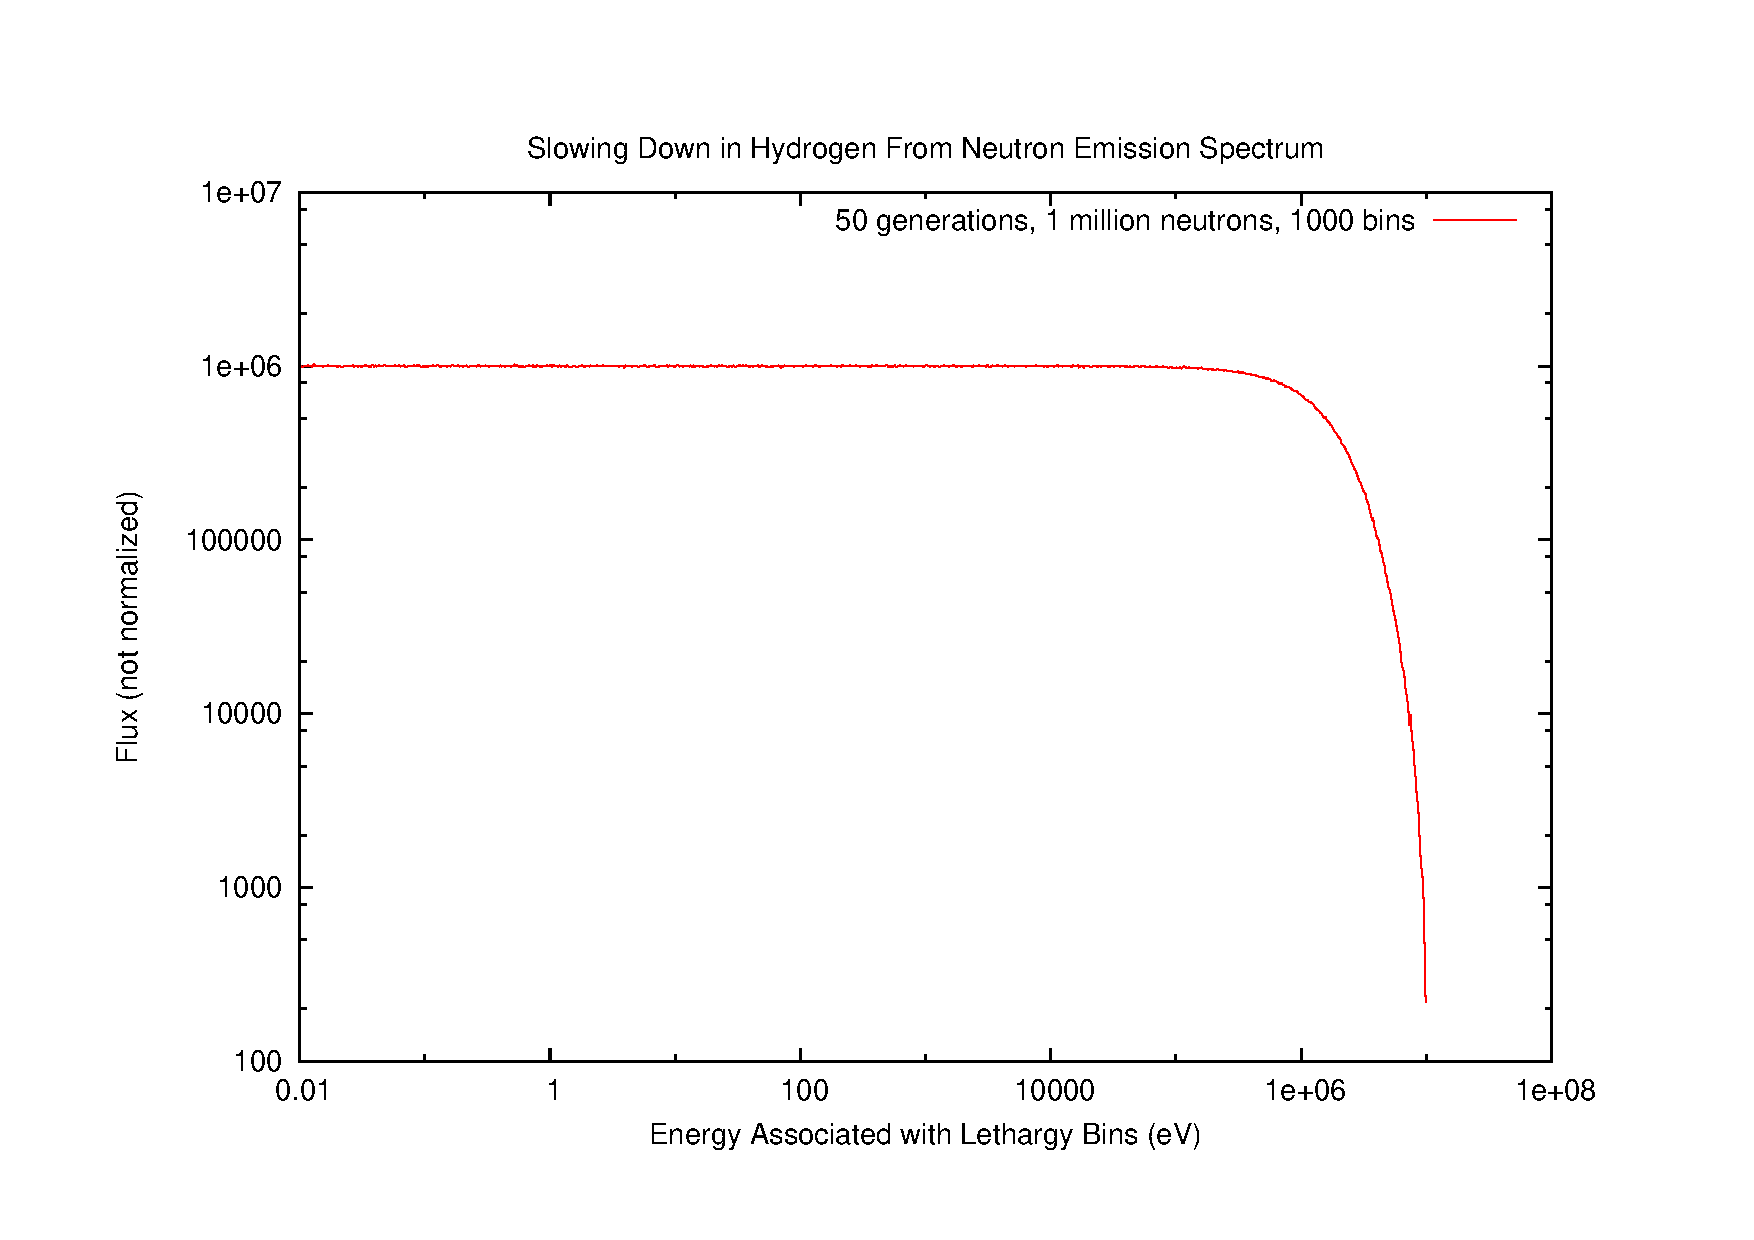
\includegraphics[width=4in]{images/sl-d/spec-2.uncrop.pdf}
  \\
  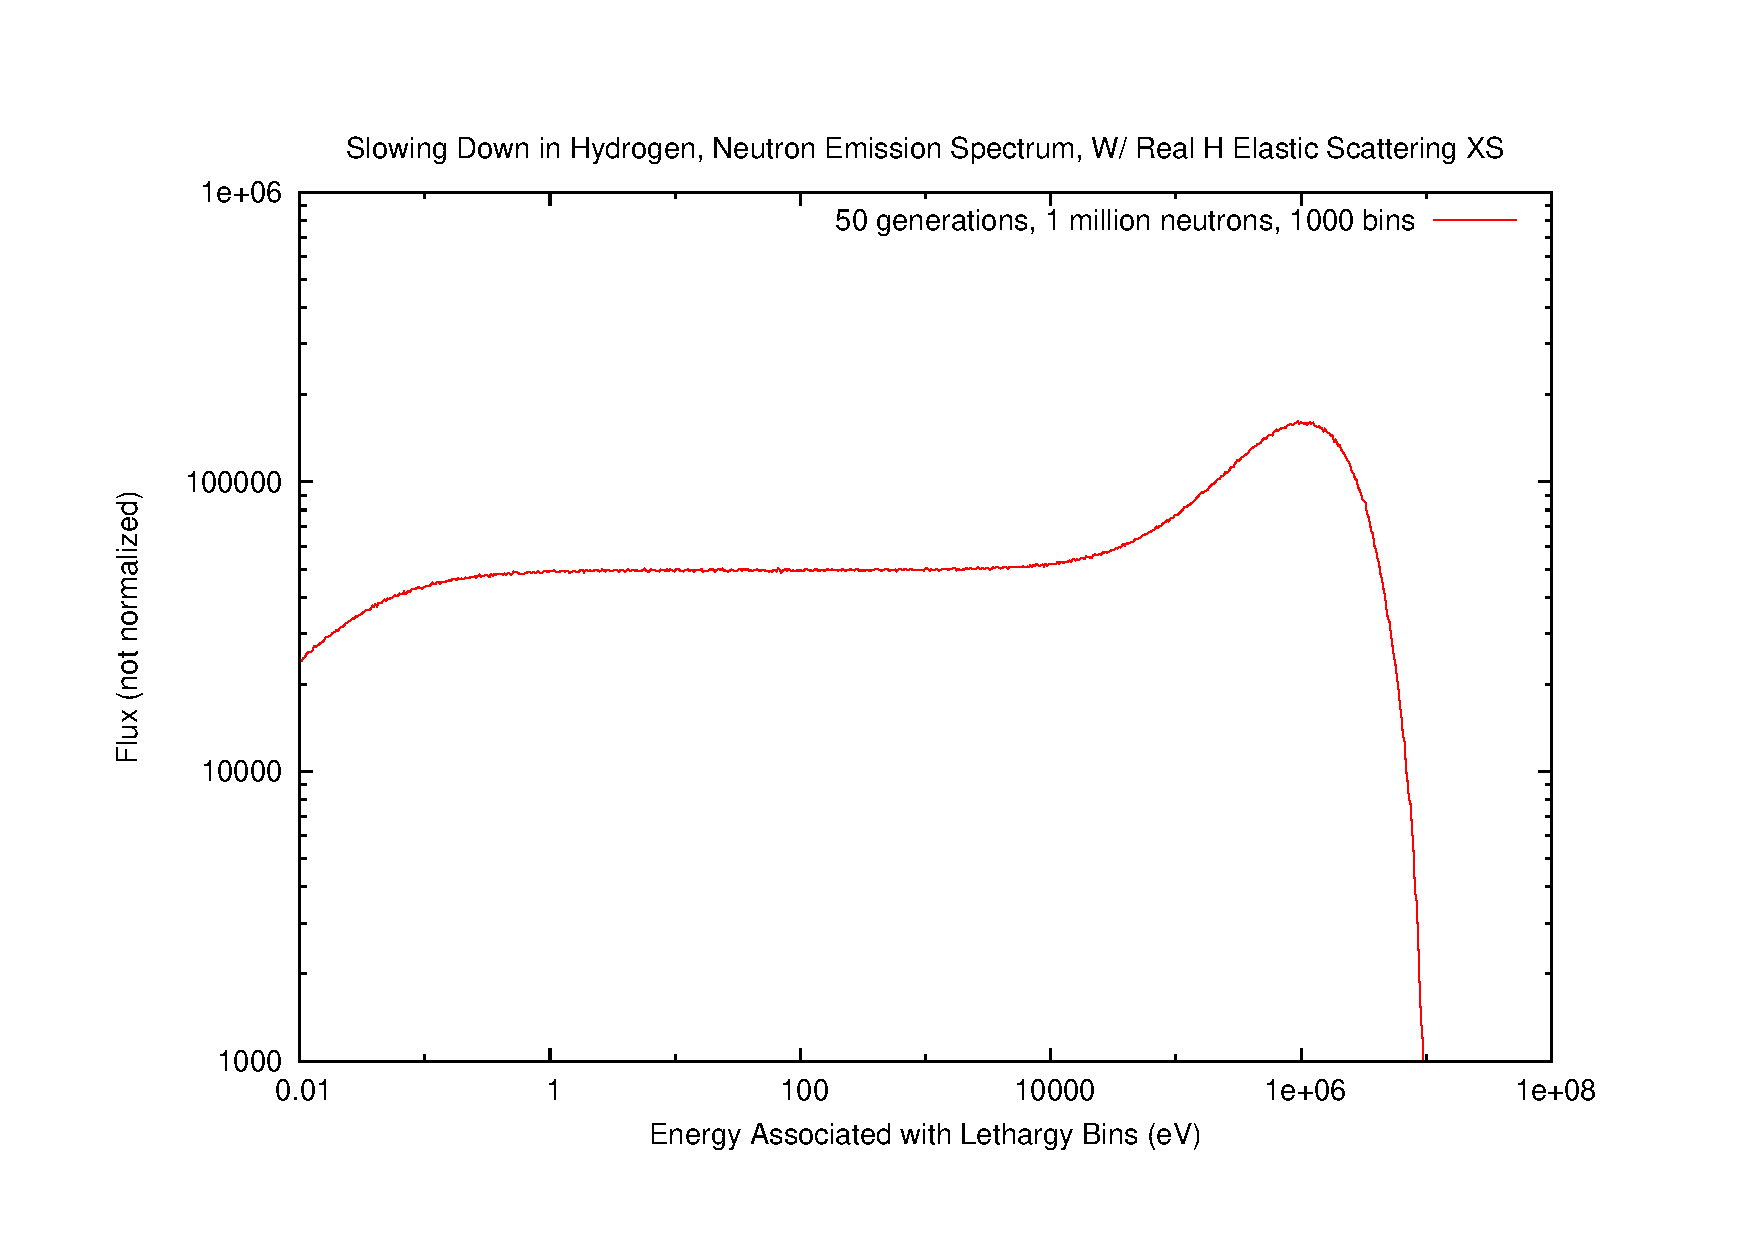
\includegraphics[width=4in]{images/sl-d/spec-3.uncrop.pdf}
  \caption{Spectrum, Added in Fission Neutron Emission Spectrum and Hydrogen Scattering XS} \label{spe1}
\end{figure}




\clearpage
\subtopic{Thermal Energy ($<4$ eV): Equilibrium Thermal Scattering}
For the thermal energy range, we are going to start with elastic scattering from stationary, free particle. Then we would consider the effects of having the target in motion and adding chemical bound.
\begin{enumerate}
\item We make three assumptions for the thermal energy range, 
  \begin{itemize}
  \item A monatomic free gas, that is, a Maxwellian distribution. 
  \item The target is at rest. 
  \item The target is free from chemical bonds. 
  \end{itemize}

Then the elastic scattering cross section dependent on $A$, $E$, and temperature $T$:
\begin{align}
  \sigma(E) f_s (E \to E') = &\frac{\sigma_{s0} \eta^2}{2E} \left[ \erf{\eta \sqrt{\frac{E'}{kT}} - \rho \sqrt{\frac{E}{kT}} } \mp \erf{\eta \sqrt{\frac{E'}{kT}} + \rho \sqrt{\frac{E}{kT}} } \right. \notag \\
    & \left. + e^{\frac{E - E'}{kT}} \left( \erf{ \eta \sqrt{\frac{E}{kT}} - \rho \sqrt{\frac{E'}{kT}} }  \pm \erf{\eta \sqrt{\frac{E}{kT}} + \rho \sqrt{\frac{E'}{kT}} } \right) \right] 
\end{align}
where the upper signs are for $E' > E$< and the lower signs for $E' < E$, and the $\eta, \rho$ terms are:
\eqn{ \eta &= \frac{A+1}{2 \sqrt{A}} & \rho &= \frac{A-1}{2 \sqrt{A}} }

\item For a proton gas (A=1), we can simplify the energy transfer function to be,
\begin{align}
\sigma_s(E) f_s(E\to E') = \frac{\sigma_{s0}}{E} \left\{ 
\begin{array}{cc}
e^{\frac{E-E'}{kT}} \erf{\sqrt{\frac{E}{kT}}} & E' > E \\
\erf{\sqrt{\frac{E'}{kT}}} & E' < E 
\end{array}
\right.
\end{align}

\begin{figure}[ht]
  \centering
  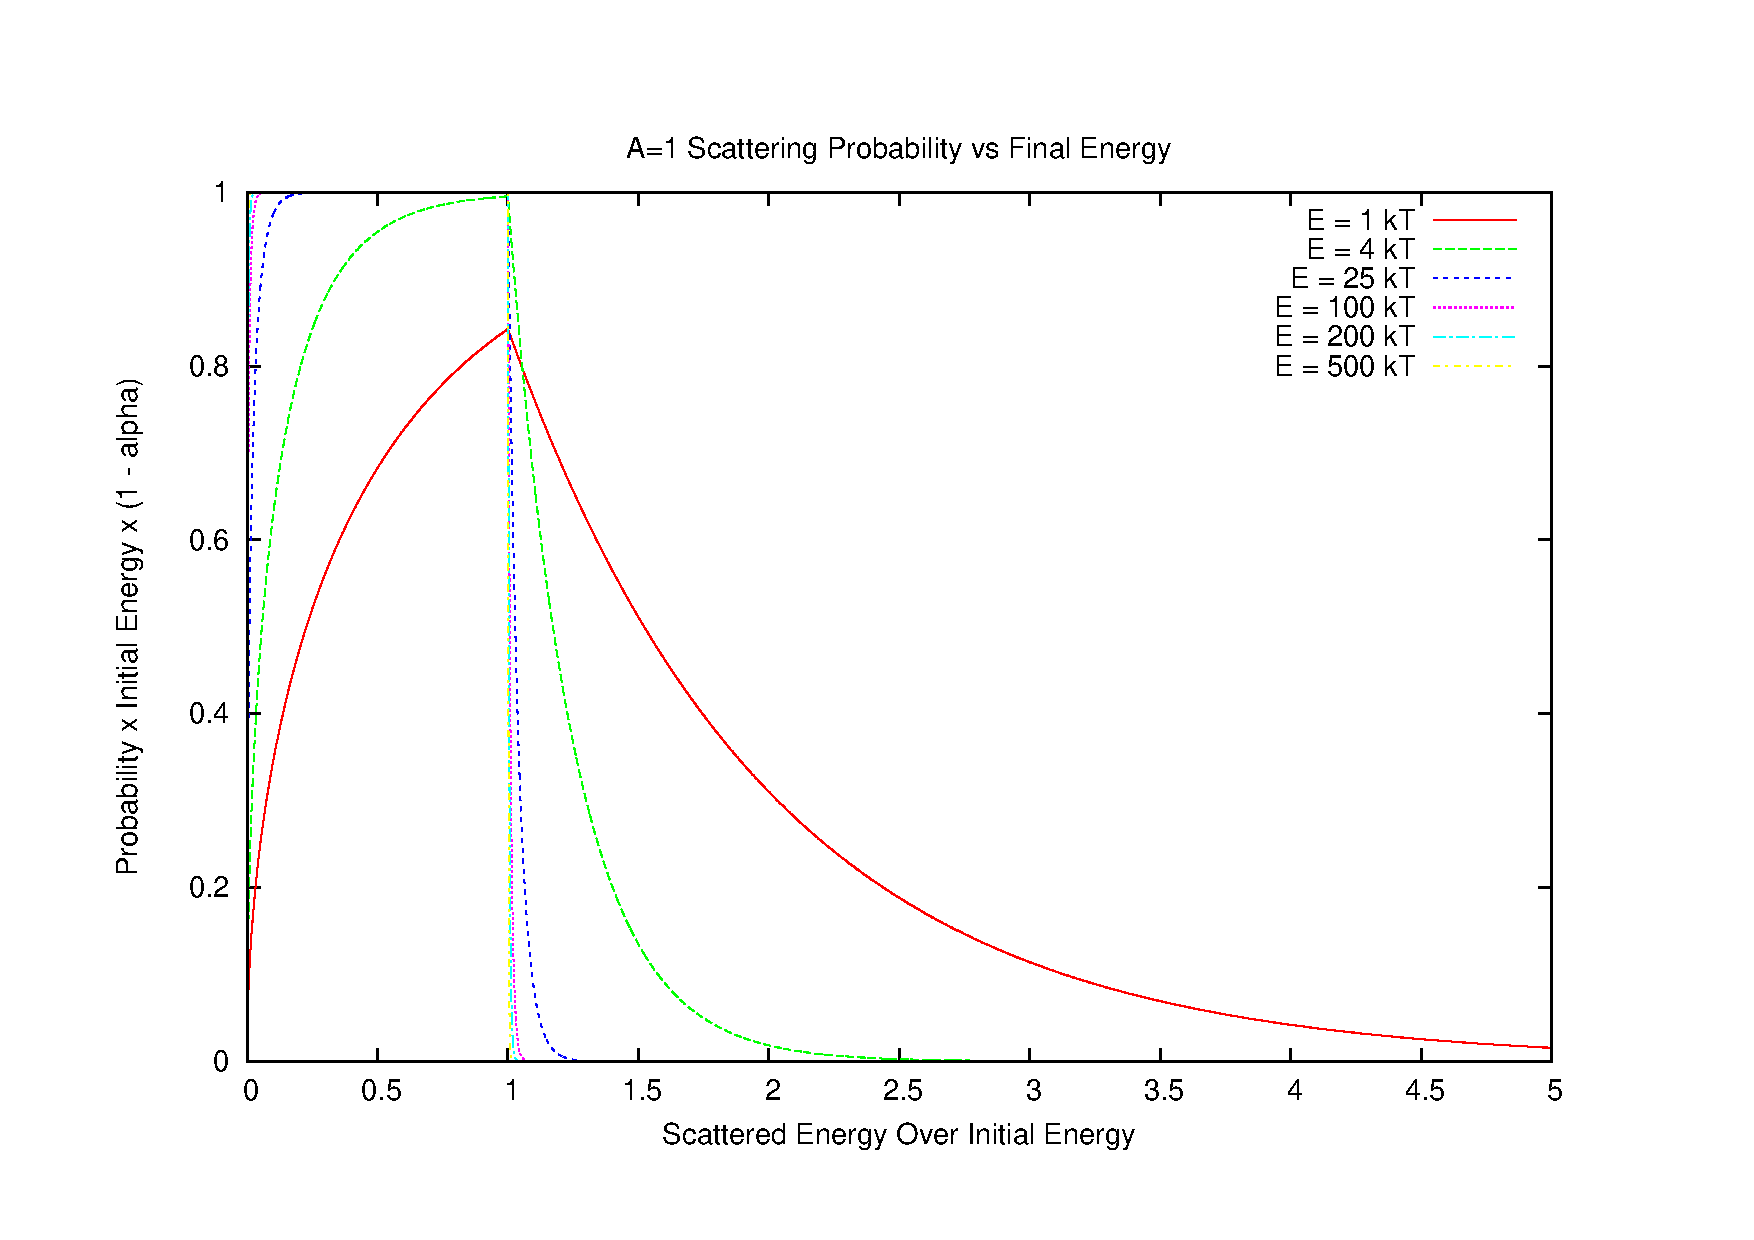
\includegraphics[width=3in]{images/sl-d/ts_H.uncrop.pdf}
  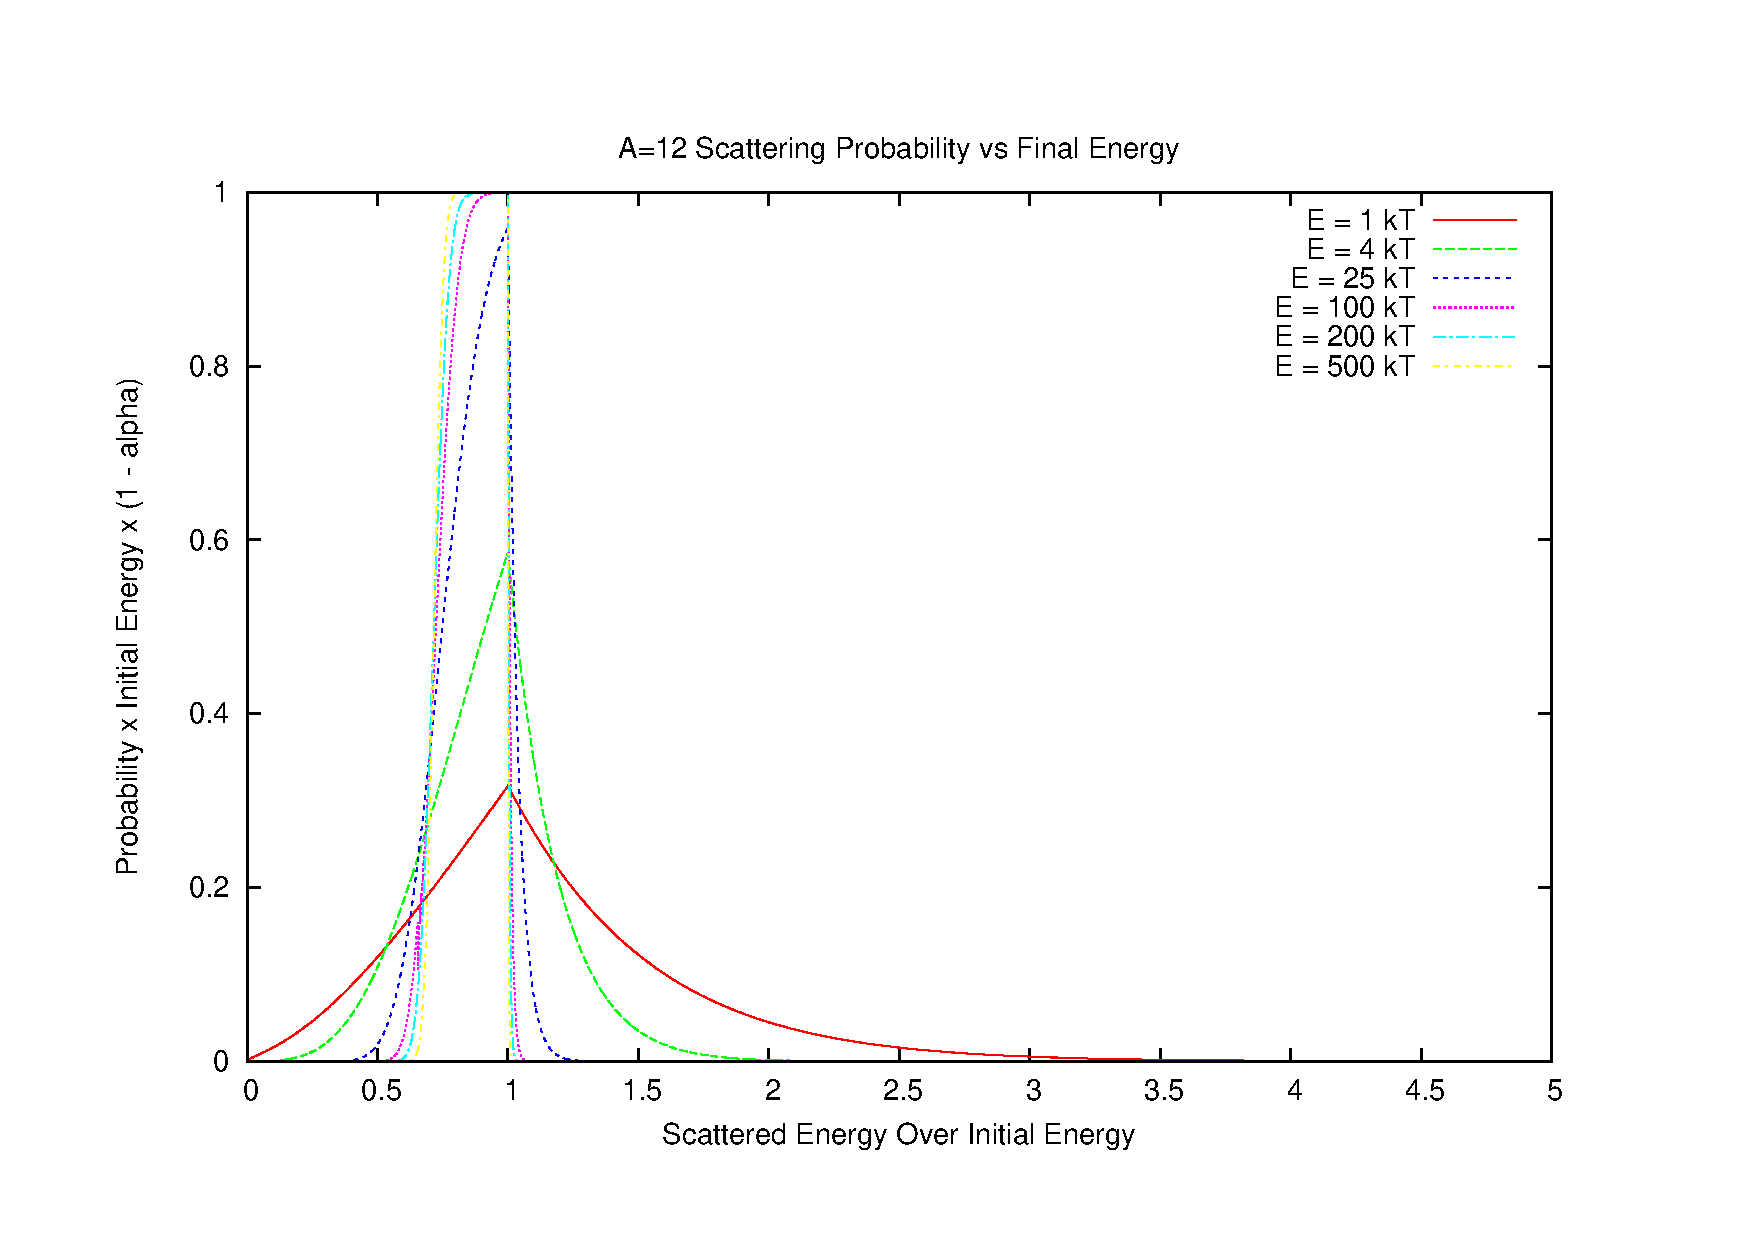
\includegraphics[width=3in]{images/sl-d/ts_C.uncrop.pdf}
  \caption{Thermal Scattering Probability vs. Energy for Hydrogen and Graphite} \label{ts-C-H}
\end{figure}
Observations: 
\begin{enumerate}
\item In Fig.~\ref{ts-C-H}: E = 1kT to 25kT provides a good cover of range, and even at 1200K, 1kT = 0.1 eV, and 25kT = 2.5eV, so 4eV is a typical upper scattering cutoff. 

\item In Fig.~\ref{ts-C-H}: the $\frac{E'}{E}$ axis shows that there is a good probability that the neutron would gain energy from the elastic scattering(the lower the initial neutron energy, the closer it is to the target nuclei thermal agitation, the more probable is upper scattering). In fact this is the difference between this thermal energy model and the previous high-energy model.  


\item We can add the thermal scattering into our MC model and observe a peak in the thermal range as in the left plot of Fig.~\ref{spe2}. To make the height more realistic, we add in the hydrogen absorption cross section (a $1/v$ distribution, only affect the thermal range) as in the right plot of Fig.~\ref{spe2}. The absorbing strength is picked such that the absorption-to-scattering ratio is something reasonable, like 0.2. 
\begin{figure}[ht]
  \centering
  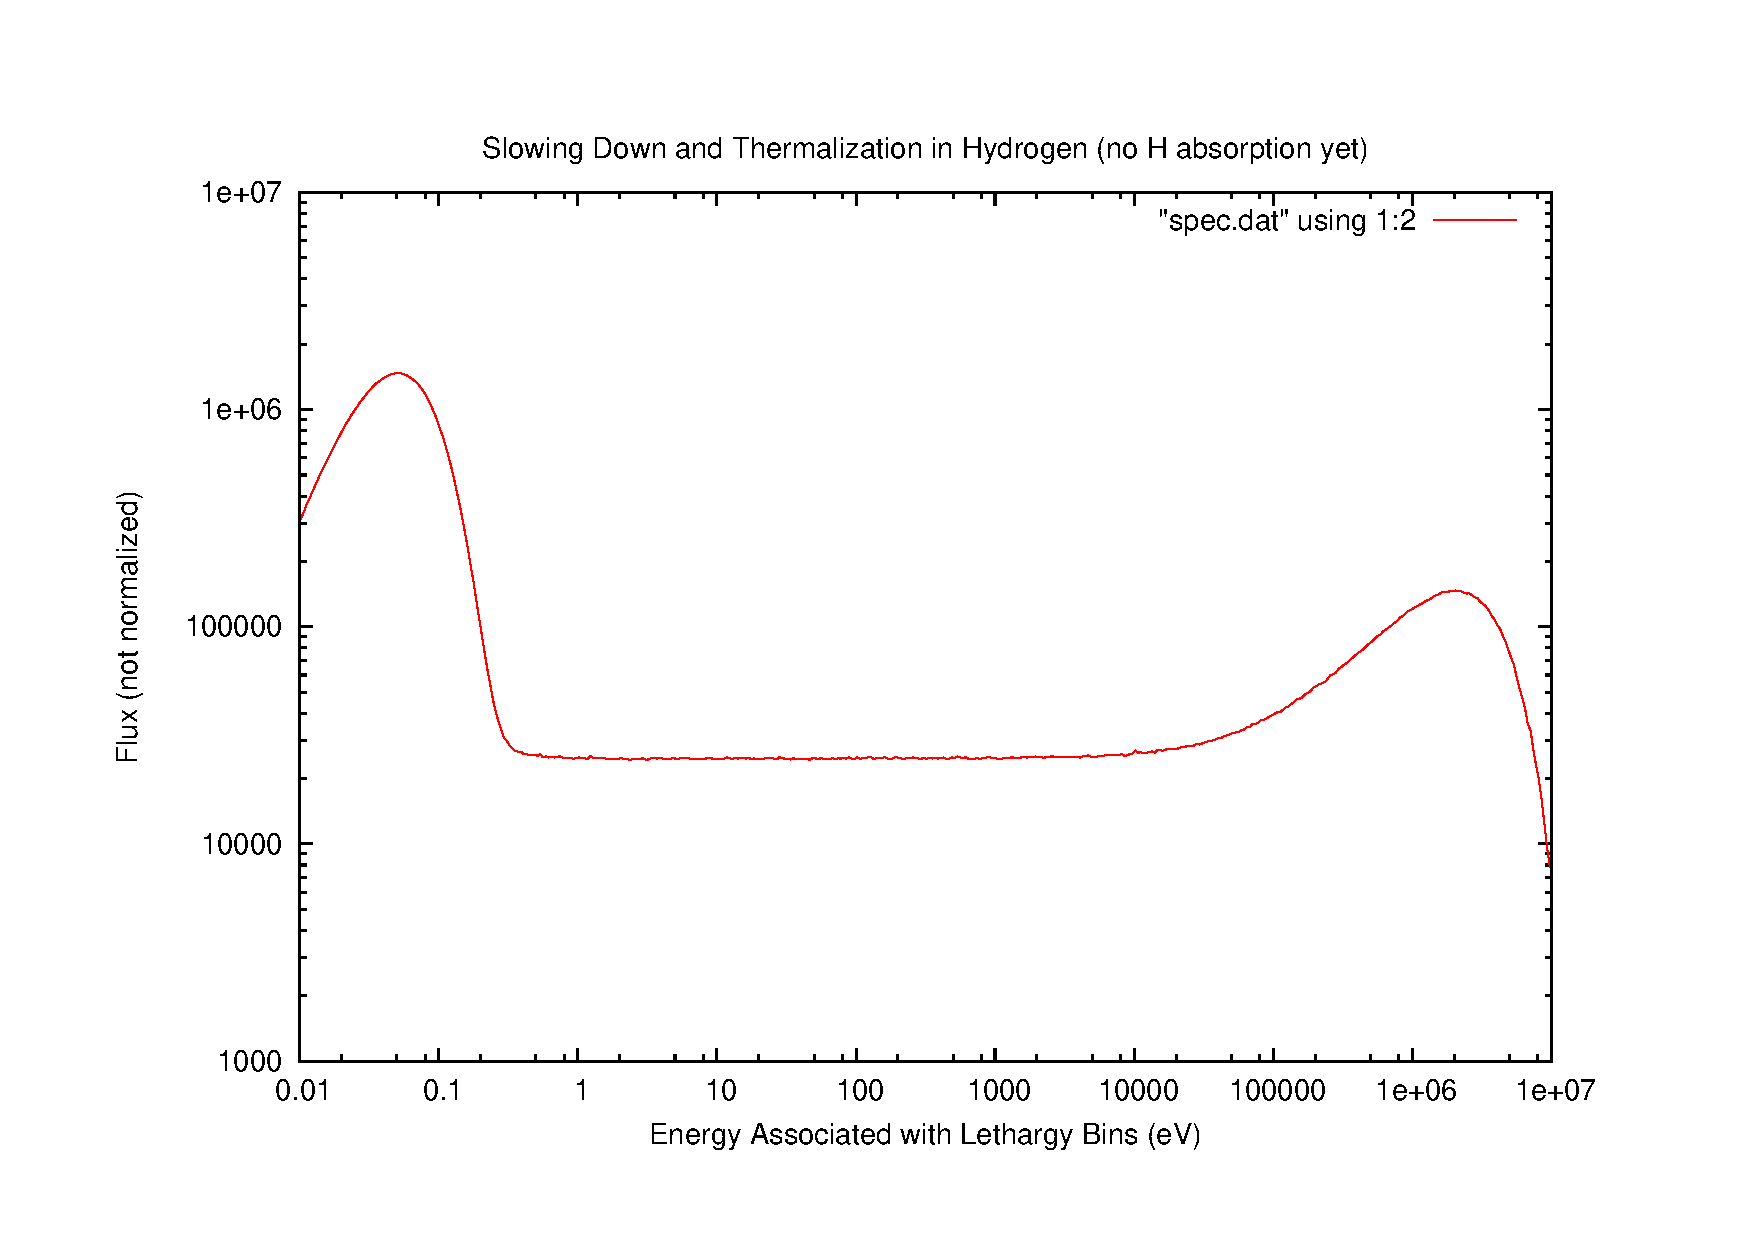
\includegraphics[width=3in]{images/sl-d/spec-4.uncrop.pdf}
  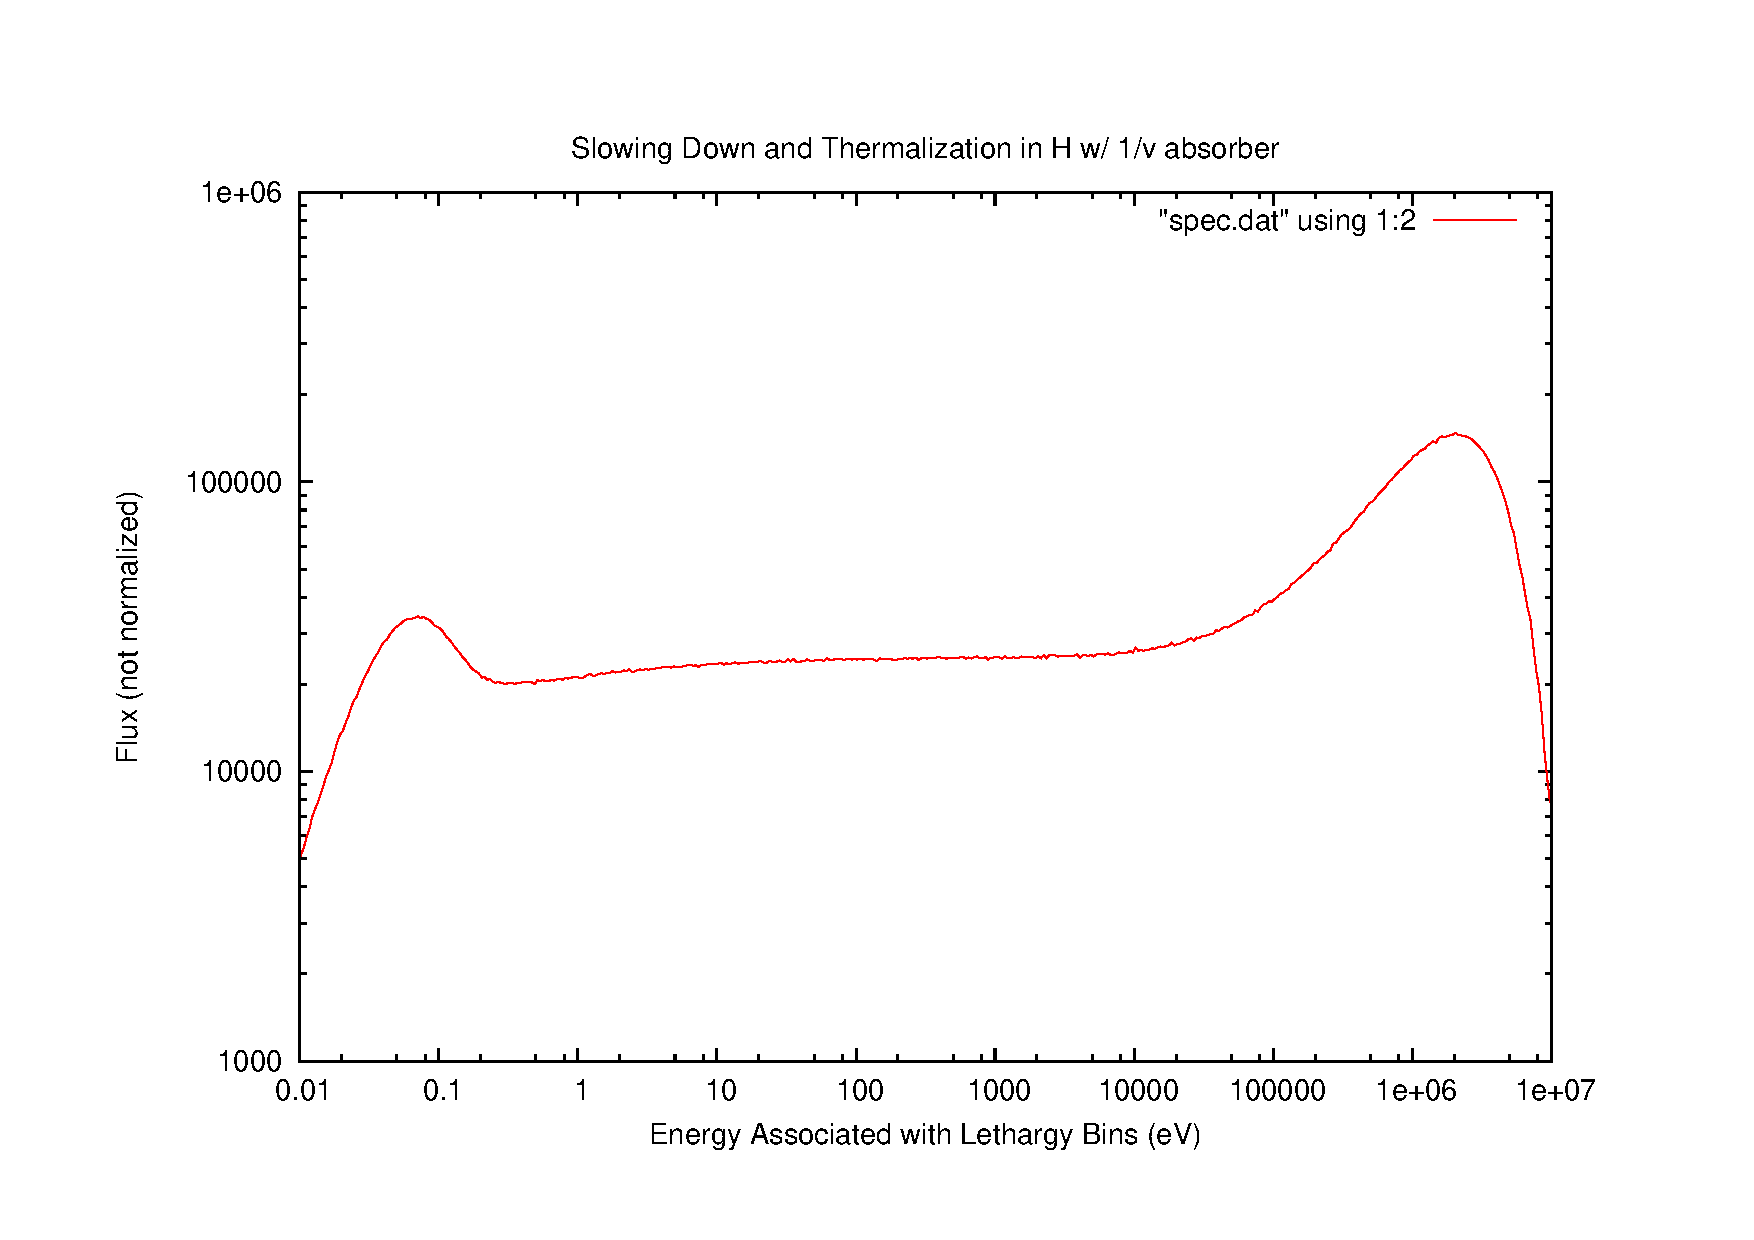
\includegraphics[width=3in]{images/sl-d/spec-5.uncrop.pdf}
  \caption{Spectrum, Added in Thermal Scattering and $1/v$ Hydrogen Absorption XS} \label{spe2}
\end{figure}
\end{enumerate}

\item Adding Target in Motion (important for U238 resonances at hot fuel conditions). Thermal agitation does not matter that much for non-resonance conditions; that is, when $\dsigma/\dE$ is small, a small $\Delta v$ hence a small $\Delta E$ does not change the cross section much. This is not true anymore for U238 resonances, because when cross section changes very rapidly (especially true in the scattering cross section than the absorption cross section), target motion/thermal agitation would affect up scattering quite significantly. As shown in Figure~\ref{timr}, it could be a 10\% increase in LWR U238 Doppler.  
\begin{figure}[ht]
  \centering
  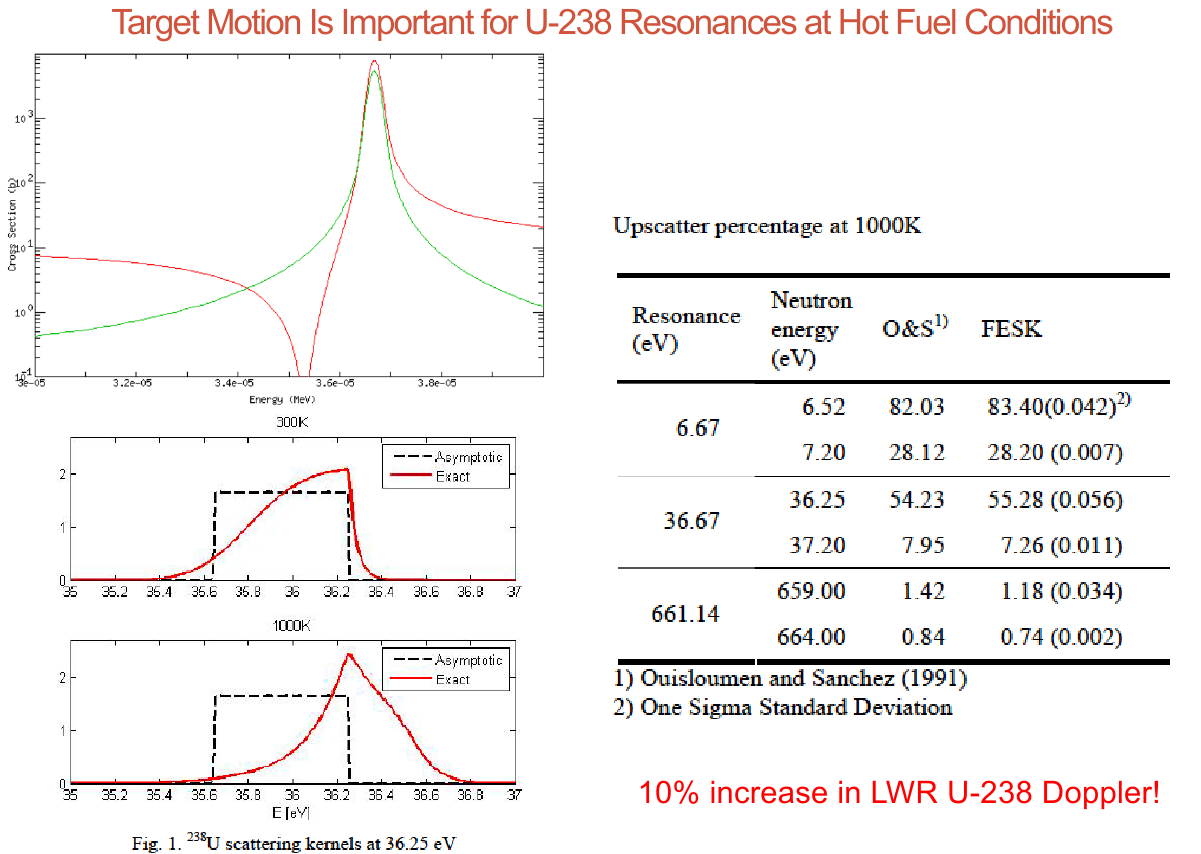
\includegraphics[width=6in]{images/sl-d/target-in-motion-resonance.png}
  \caption{Target Motion Is Important for U238 Resonances} \label{timr}
\end{figure}

We will cover resonance models later, for now we just need to know that the weird dips in scattering cross section is a result of the interacting wave between the potential scattering and the compound nuclear scattering. 

\item Adding chemical bound to get bound elastic scattering of H in \ce{H_2 O} molecules. So far we've only talked about free gas; in the case of tightly bound atoms at very low energy, the vibrations within a molecule due to the chemical bond come into play:
  \eqn{\sigma_{\mathrm{bound}} = \left( 1 + \frac{1}{A_{\mathrm{atom}}} \right) \sigma_{\mathrm{free}}  }
  For bound water molecule for instance, 
  \eqn{ \sigma_{\mathrm{water}}^H = (1+1)^2 \sigma_H = 4 \sigma_H }
  The dependency on $A$ suggests that \textit{the bound elastic scattering matters for light nuclei, and not so much for heavy nuclei}. In the case of hydrogen, the free gas model would still provide the right shape, but the probability can be off by a factor of 10. In the case of graphite, the free gas model does not provide the right shape. The lower energy you want to go, the more careful you need to be. 

  Elastic scattering for bound molecules can be characterized by,
  \eqn{ \frac{\derivative^2 \sigma}{\dOmega \dE'} (E\to E', \Omega\to \Omega')  = \frac{\sigma_b}{4 \pi kT} \sqrt{ \frac{E'}{E}} e^{-\frac{\beta}{2}} S(\alpha, \beta)   }
  where $\sigma_b$ is the bound scattering cross section for the material, $kT$ is in eV, $S(\alpha, \beta)$ is the symmetric form of the thermal scattering law, since $\alpha, \beta$ depends on temperature, $S$ depends on temperature too. 
  \eqn{ S(\alpha, \beta) = \frac{\exp{-\frac{\alpha^2 + \beta^2}{4 \alpha}} }{\sqrt{4\pi \alpha}} }
  where $\alpha, \beta$ depends on two terms:
  \begin{itemize}
  \item The momentum transfer $\kappa$,
    \eqn{ \alpha = \frac{E' + E - 2 \sqrt{E' E} \cos \theta}{A kT} = \frac{\hbar^2 \kappa^2}{2 M kT} } 
    where $A$ is the ratio of the mass of the scattering atom to the neutron mass.
  \item The energy transfer $\epsilon$,
    \eqn{ \beta = \frac{E' - E}{kT} = \frac{\epsilon}{kT} }
  \end{itemize}

\item Recap: 
  \begin{itemize}
  \item Thermal scattering distributions: generate cdf for energies, like from 0.1kT to 8kT.  
  \item 4 eV is the typicall up-scattering cutoff energy. For an incident neutron energy higher than 4 eV, use asymptotic elastic down scattering. 
  \end{itemize}
\end{enumerate}
%%%%%%%%%%%%%%%%%%%%%% start of MC %%%%%%%%%%%%%%%%%%%%%%%%%%%%%


%%%%%%%%%%%%%%%%%%%%%%% start of Analytical %%%%%%%%%%%%%%%%%%%%%%%%%%%%%%
\clearpage
\topic{Analytical Derivation} \label{slowing-down-from-te}
\subtopic{Derivation from TE} 
This lecture is given on Oct. 2 by Prof. Forget. We start from the TE: 
\eqn{ \frac{1}{v} \pphipt + \Omega \gradient \phi + \Sigma_t \phi &= \int \dE \int \dOmega \Sigma_s \phi + \frac{\chi(E)}{4 \pi} \int \dE v \Sigma_f \phi + S }
Apply assumptions:
\begin{enumerate}
\item Steady state, so $\frac{1}{v} \pphipt \to 0$. 
\item Infinite medium, so no streaming term $\Omega \gradient \phi \to 0$. 
\item No source, so $S \to 0$. 
\item Slowing down happens through elastic scattering that is isotropic in the center of mass system (s-wave elastic scattering), that is, 
  \eqn{ \Sigma_s (E' \to E) &= \frac{\Sigma_s(E')}{(1-\alpha)E'} &\mbox{for } E < E' < \frac{E}{\alpha} }
  where $\alpha = (A-1/A+1)^2$. In assuming s-wave, the slowing down model only applies for neutrons below 1MeV in light moderators and neutrons below 0.1 MeV in heavier materials, since the average $\bar{\mu_0} = 0.07 A^{2/3}E$ [MeV].  For neutrons above 0.1 MeV, inelastic scattering from heavy nuclei becomes important and cannot be ignored (but I don't think we've ever addressed inelastic scattering in this course).
\end{enumerate}

When we had the time dependent term $\pphipt$, flux changes with respect to time and is driven by source. Once we go into steady state and take away the source, \textbf{TE becomes an eigenvalue problem, and we need to add a $k$ on the bottom of the fission term}. Notice that our TE only depends on energy now,  
\eqn{ \Sigma_t (E) \phi(E) &= \int_0^{\infty} \dE' \Sigma_s (E'\to E) \phi(E') + \frac{\chi(E)}{k} \int_0^{\infty} \dE' \nu(E') \Sigma_f(E') \phi(E') }
If we re-write assuming the fission source is an external source of neutrons $S_f$ (notice it's energy independent): 
\eqn{ \Sigma_t(E) \phi(E) &= \int_0^{\infty} \dE' \Sigma_s (E' \to E) \phi(E') + \chi(E) S_f }
where we can subsitute $P(E'\to E) = \frac{1}{(1-\alpha)E'}$ into $\Sigma_s(E' \to E) = \Sigma_s(E') P(E' \to E)$. Alternatively we can write the TE in lethargy space: 
\eqn{ \Sigma_t(u) \phi(u) = \int_{-\infty}^u \Sigma_s(u \to u') \phi(u') \du' + \chi(u) S_f }

\begin{enumerate}
\item Fast range ($>0.1$MeV): Assume no upscattering, and any scattering event is likely to slow neutrons below 0.1 MeV. Then our TE becomes, 
  \eqn{ \Sigma_t (E) \phi(E) &= \chi(E) S_f  & \Aboxed{\phi(E) &= \frac{\chi(E) S_f}{\Sigma_t} } }
 \hi{$\chi(E)$ dominantes fast flux}, because $\Sigma_t$ is fairly flat in the fast range, and $S_f = \frac{\nu \Sigma_f \phi}{k}$ which is proportional to $\phi(E)$ anyway (or say flux scales with source), so we are left with the distribution of prompt neutrons dominant the flux in the fast range. 

\item Slowing down region/resonance region $[1\eV, 0.1 \MeV]$. We define a slowing down density: 
  \eqn{ q(E) = \mbox{ number of minimum slowing down past energy }E}
  Again assume no upscattering. In the presence of scattering, all neutrons born from fission will reach $E$ unless absorbed, 
  \eqn{ q(E) = \int_E^{\infty} \chi(E') S_f \dE' - \int_E^{\infty} \Sigma_a(E') \phi(E') \dE' }
  From the general expression $\int_0^{\infty} \chi(E') \dE' = 1$, we can approximate $\int_{0.1}^{\infty} \chi(E') \dE' = 1$, thus only leaving the energy independent $S_f$ term:  
  \begin{align}
    q(E) &= - \int_E^{\infty} \Sigma_a (E') \phi(E') \dE' + S_f \\
    \Aboxed{ \frac{\derivative q(E)}{\dE} &= - \Sigma_a (E) \phi(E) } 
  \end{align}
  Comments/notes: 
  \begin{itemize}
    \item If absorption increases, less neutrons would make it to $E$, then $q(E)$ should be smaller. 
    \item $q(E)$ decreases proportional to $\Sigma_a$, because in our approximation the source term becomes indpendent of energy. 
    \item If $\Sigma_a = 0, q(E) = $ constant. 
  \end{itemize}

In reactor applications, most absorptions happen in the resonances of \ce{^{238} U}. \ce{^{238}U}'s cross section changes by order of magnitudes for each resonance, so we can assume that $\Sigma_a = 0$ between resonances (also because between resonances there is no quantum effect between compound nuclides). That is, $q(E)=$ constant between resonances. Consider our TE again with $\Sigma_a = 0$, 
      \eqn{ \Sigma_s (E) \phi(E) = \int_0^{\infty} \Sigma_s (E'\to E) \phi(E') \dE' }
      Plug in $\Sigma_s (E' \to E) = \Sigma_s (E') P(E' \to E) = \frac{\Sigma_s (E')}{(1-\alpha) E'}$. Also assume: below birth $E$ of fission neutrons, below inelastic scattering threshold, single scattering nuclei, 
      \eqn{ \Sigma_s (E) \phi(E) = \int_0^{E/\alpha} \frac{1}{(1-\alpha)E'} \Sigma_s (E') \phi(E') \dE' }
      We know (magically) that the solution of the above integral is of the form, 
      \eqn{ \Sigma_s (E) \phi(E) = \frac{\mbox{C}}{E} }

      \begin{figure}[ht]
        \centering
        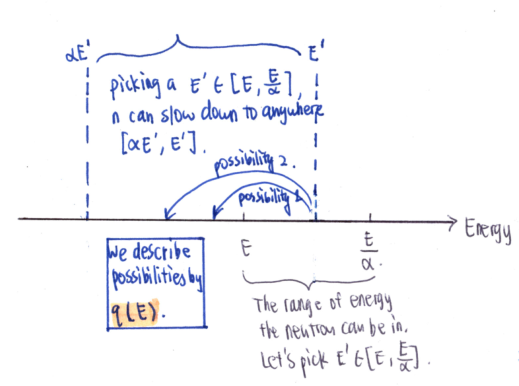
\includegraphics[width=4in]{images/sl-d/sl-d-energy.png}
        \caption{Slowing Down in Energy} \label{sl-d-energy}
      \end{figure}

      Motivated by Fig.~\ref{sl-d-energy}, we define $q(E)$ in terms of scattering, 
      \eqn{ q(E) = \int_E^{E/\alpha} \left[ \int_{\alpha E'}^{E'} \frac{1}{(1-\alpha) E''} \Sigma_s(E'') \phi(E'') \dE'' \right] \dE' } 
      Plug in $\Sigma_s \phi = C/E$, integrate twice, we get, 
      \eqn{ q(E) = \left[ 1 + \frac{\alpha}{1-\alpha} \ln \alpha \right] C = \xi C }
      Consider $\Sigma_s (E) \phi(E) E = C$, that is $q(E) = \xi \Sigma_s (E) \phi(E) E$, we reach \footnote{a subtle point here is that the equations here are the asymptotic values. Recall the Placzek Transient is due to the discontinuity of the flux at $u = \epsilon$, and its derivative at $u = 2 \epsilon$ etc where $\epsilon$ is the maximum lethargy gain. The discontinuity is more noticable for heavy nuclides, and disappear for hydrogen.}, 
      \eqn{ \Aboxed{ \phi(E) &= \frac{q(E)}{\xi \Sigma_s (E) E} }  & \phi(u) &= \frac{q(u)}{\xi \Sigma_s (\mu)  } }

      \begin{figure}[ht]
        \centering
        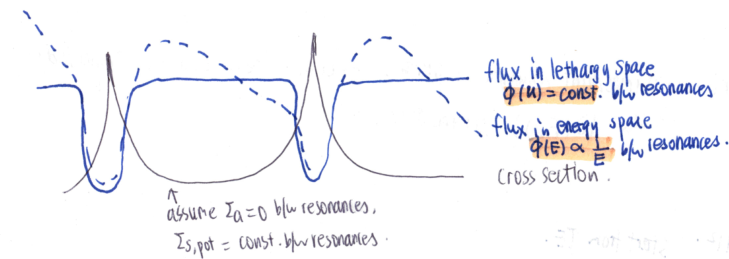
\includegraphics[width=6.5in]{images/sl-d/resonance-flux.png}
        \caption{Flux Between Resonances} \label{resonance-flux}
      \end{figure}
\end{enumerate}

\subtopic{Convolution of 0K Cross Section} % 10/18/12 
So far in our slowing down derivation, we have implicitaly assumed that the target is at rest. In reactor applications, thermal agitation is always present for the temperature of interest, and it increases as temperature increases. Thus we need to account for the relative energy between the neutron and the target. 

We call $V_A$ the atom velocity, $V_n$ the neutron velocity, then the relative velocity is $V_R = V_n - V_A$. The convolution of 0K cross section is leads to \hi{the convolution integral}, 
\eqn{ \bar{\sigma}_x(V_n) = \frac{1}{V_n} \int \derivative^3 v_a p(V_A) |V_n - V_A| \sigma_x (|V_n - V_A|) }
where $p(V_A)$ is the Maxwellian distribution, and the $\sigma_x(|V_n - V_A|)$ is the 0K cross section at the corrected velocity $V_n - V_A$. 

Essentially we `correct' the cross section using an average velocity distribution of the material at temperature T. The effect on resonance range is, 
\begin{itemize}
\item Resonances broaden as temperature increases. 
\item The higher the temperature, the smoother the resonance would be, the smoother the cross section would be. 
\item Resonances nearer to the thermal region would broaden more than resonances near the fast range. 
\end{itemize}

In the thermal range, the convolution of a constant cross section would increase the thermal cross section as temperature increases; more specifically, scattering cross section tends to be constant in low temperature, and becomes 1/v as temperature increases; thus at higher temperatures it is harder to tell absorption cross section (1/v) and scattering cross section apart. 

Prof. Forget introduces SLBW here. \textcolor{blue}{The convolution integral will yield the expression in section 2.7.1 with Psi, Chi definitions of 8.4.3}. 

$\Psi$ term shows up in both absorption and scattering cross section terms and it gives the shape of the cross section. $\Chi$ term only shows up in the scattering cross section and it represents the interference effect. The sum of $\Psi$ and $\Chi$ results in the dip before peaking that always shows up in the scattering cross section. 


%%%%%%%%%%%%%%%%%%%%%%% end of Analytical %%%%%%%%%%%%%%%%%%%%%%%%%%%%%%


\clearpage
\topic{Summary}
\begin{enumerate}
\item Properties of isotropic elastic scattering/asymptotic downscattering (which we assume for larger than 4 eV). See Table.~\ref{slowing-down-parameter} for common values. 
  \begin{enumerate}
    \item After each collision, the minimum energy is characterized by: 
      \eqn{ \alpha = \frac{E_{\mathrm{min}}}{E_0} = \left( \frac{A-1}{A+1} \right)^2 }
      
    \item Mean log energy decrement: $A \up, \xi \down$. 
      \eqn{ \xi = 1 + \frac{\alpha}{1-\alpha} \ln \alpha} 

    \item Number of collisions required to slow a particle from $E_i$ to $E_f$:
      \eqn{ n = \frac{\ln(E_i/E_f)}{\xi} }
  \end{enumerate}

\item Not near sources or resonance (Duderstadt p.319): 
  \eqn{ \Phi(u) \sim \frac{1}{\Sigma_s(u)} }

\item Fast energy range, $\chi(E)$ dominantes flux:
  \eqn{ \Phi(E) = \frac{\chi(E) S_f}{\Sigma_t(E)} }

\item Resonance energy range: 
  \begin{enumerate}
    \item Assumptions: between resonances $\Sigma_a =0$, and $\Sigma_s$ = constant (the compound nuclide scattering cross section is again zero because no QM between nuclides, potential scattering is constant around $4 \pi R^2$). 

    \item Collision rate density 
      \eqn{ F(E) = \Sigma_s (E) \Phi(E) }
      It is discontinuous for non-hydrogen atoms at $\alpha^n E_0$ which are the minimum energy a neutron can slow down to in the $n$-th collision. 

    \item Slow down density $q(E)$: \# neutrons crossing the boundary. $q(E)$ depends on: neutrons born (if no absorption, all neutrons born would all cross boundary at some point), and absorption: 
      \eqn{ q(E) = \int_{u-\ln(1/\alpha)}^u \du' F_c (u') \int_u^{u'+\ln (1/\alpha)} \du'' \frac{e^{u' - u''}}{1-\alpha} }
      We can reach an general expression for $q(E)$:
      \eqn{ \frac{\dq(E)}{\dE} =  - \Sigma_a (E) \Phi(E) }

    \item If we further assumes there is no absorption at all, all source $S_0$ eventually slow down to $E$. $F(E)$ would eventually reach it's asymptotic solution of: 
      \eqn{ F(E) &\to \frac{S_0}{\xi E}   & F(u) &\to \frac{S_0}{\xi} }
      \eqn{\Aboxed{q(u) &= S_0} & \Aboxed{ \Phi(u) &= \frac{S_0}{\xi \Sigma_s(u)}}}
  \end{enumerate}
\end{enumerate}






\end{document}
